\section{Lecture 23}
\subsection{Lecture Notes - Hamiltonian Mechanics}
\subsubsection{Hamilton's Equations \& Properties}
A particle slides on a helical wire defined by $z = k\theta$, $r = R$. If we use $\theta$ as the generalized coordinate, the generalized momentum is $p = m(r^2 + k^2)\dot{\theta}$. What is the Hamiltonian of the system?
\begin{s}
    Using the fact that here the Hamiltonian is equal to the energy:
    \[\mathcal{H} = T + U = \frac{p^2}{2m} + mgk\theta\]
\end{s}
Last lecture, we derived Hamilton's equations of motion:
\[\boxed{\dpd{\mathcal{H}}{p_i} = \dot{q}_i, \quad \dpd{\mathcal{H}}{q_i} = - \dot{p}_i}\]
This was done by starting with the Hamiltonian (Legendre transform of $\mathcal{L}$), expanding out in the total differential of $\mathcal{H}$, then using the EL equation to solve for Hamilton's equation (see last day's notes for more detail). We notice that Hamilton's equations are two first order equations, rather than a single second order equation. In general, if we have $n$ degrees of freedom, the Lagrangian gives us $n$ 2nd order differential equations, while Hamilton gives us $2n$ 1st order differential equations. 

\noindent Now suppose that the Hamiltonian is independent of $p_i$. What can we say about the system?
\begin{s}
$q_i$ is constant by Hamilton's equations.
\end{s}

Now, what do Hamilton's equations tell us about the derivatives $\dpd{\dot{q}_i}{q_i} + \dpd{\dot{p}_i}{p_i}$?
\begin{s}
Again using Hamilton's equation, these are equal to:
\[\dpd{\HH}{q_ip_i} - \dpd{\HH}{p_iq_i} = 0\]
By the equality of mixed partials.
\end{s}

\subsubsection{The Variational Principle, Revisited}
From Lagrangian mechanics, we have that the variation in the action is zero:
\[\delta S = \delta \int_{t_1}^{t_2}\mathcal{L}dt = \delta \int_{t_1}^{t_2}[\sum p_i\dot{q}_i - \mathcal{H}]dt = 0\]
Expanding this, we have:
\[\int_{t_1}^{t_2}\sum_i \left[-\left(\dot{p}_i + \dpd{\HH}{q_i}\right)\delta q_i + \left(\dot{q}_i - \dpd{\HH}{p_i}\right)\delta p_i\right] dt = 0\]
What does this imply about the terms in parentheses?
\begin{s}
Since $q$ and $p$ can be varied independently, both $\dot{p}_i + \dpd{\HH}{q_i}$ and $\dot{q}_i - \dpd{\HH}{p_i}$ must vanish independently; these are exactly Hamilton's equations of motion!
\end{s}

\subsubsection{Hamiltonian Time Dependence}
Let us now look at the time derivative of the Hamiltonian:
\[\dod{\mathcal{H}}{t} = \sum_i\left(\dpd{\mathcal{H}}{q_i}\dot{q}_i + \dpd{\HH}{p_i}\dot{p}_i\right)  + \dpd{\HH}{t}\]
Assuming the trajectory obeys Hamilton's equations, we have:
\[\dod{\mathcal{H}}{t} = \sum_i\left(-\dot{p}_i\dot{q}_i + \dot{q}_i\dot{p}_i\right) + \dpd{\HH}{t} = = \dpd{\HH}{t} = - \dpd{\LL}{t} \]
Even though $\HH$ is a function of $q, p, t$, the only explicit time dependence comes from the Hamiltonian itself! $\HH$ is constant if $\LL$ is independent of time.

\subsubsection{The Atwood Machine, Again}
\begin{center}
    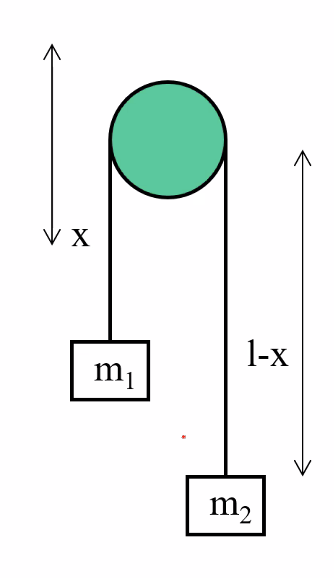
\includegraphics[scale=0.5]{Lecture-23/l23-img1.png}
\end{center}
The Atwood machine has Hamiltonian:
\[\HH = \frac{p^2}{2(m_1 + m_2)} - (m_1 - m_2)gx - m_2gl\]
What are the equations of motion?
\begin{s}
By Hamilton's equations:
\[\dot{x} = \frac{p}{m_1 + m_2}\]
\[\dot{p} = (m_1 - m_2)g\]
\end{s}
How does the system move?
\begin{s}
From above, we can see that $x$ moves with constant gravitational acceleration with effective mass \[\frac{m_1 - m_2}{m_1 + m_2}\]
Which we can see from:
\[\ddot{x} = \frac{m_1 - m_2}{m_1 + m_2}g\]
We can also reason this from limits of $m_1 \ll m_2$, $m_1 \gg m_2$.
\end{s}

\subsubsection{Phase Space of the Harmonic Oscillator}
Phase space is the set of points $\set{q_i, p_i}$ i.e. possible combinations of (generalized) position/momenta. We can write the phase space vector as $\v{z} = (\v{q}, \v{p})$. For the Harmonic oscillator in one dimension (spring constant $k$, mass $m$ distance from equlibrium $x$), we have the Hamiltonian:
\[\HH = \frac{p_x^2}{2m} + \frac{k}{2}x^2\]
Hamilton's equations give:
\[\dot{p}_x = -\dpd{\HH}{x} = -kx\]
\[\dot{x} = \dpd{\HH}{p_x} = \frac{p_x}{m}\]
Of course, we may combine these to get:
\[\ddot{x} = \frac{p_x}{m} = -\frac{k}{m}x\]
We may write Hamilton's equations as a vector:
\[\m{\dot{x} \\ \dot{p}_x} = \m{p_x/m \\ -kx}\]
We know that this will have solutions:
\[x = x_0\cos(\sqrt{\frac{k}{m}}t - \delta)\]
\[p_x = m\dot{x} = -mx_0\sqrt{\frac{k}{m}}\sin(\sqrt{\frac{k}{m}}t - \delta)\]
Now, we observe:
\[\frac{x^2}{x_0^2} + \frac{p_x^2}{mx_0^2k} = \sin^2(x) + \cos^2(x) = 1\]
But this of course is just the equation for an ellipse, that tells us that the trajectory in phase space of the harmonic oscillator will be an ellipse! In particular, which of the two directions (if both) are possible?
\begin{center}
    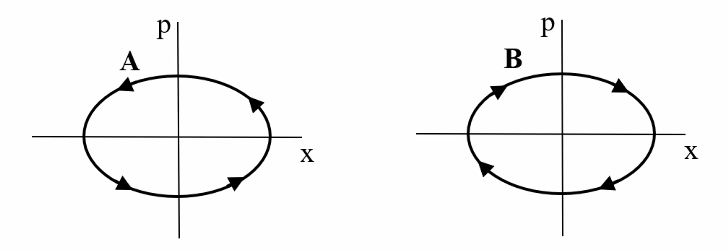
\includegraphics[scale=0.8]{Lecture-23/l23-img2.png}
\end{center}
\begin{s}
Only B; consider that when we sit at the rightmost point in the ellipse, we get pulled back towards the origin, hence the magnitude of the momentum increases, in the negative direction. Hence only the second trajectory makes sense. 
\end{s}
Now, consider a collection of harmonic oscillators which have the same energy but different relative phases. Which collection of phase points represents this system at a given instant in time?
\begin{center}
    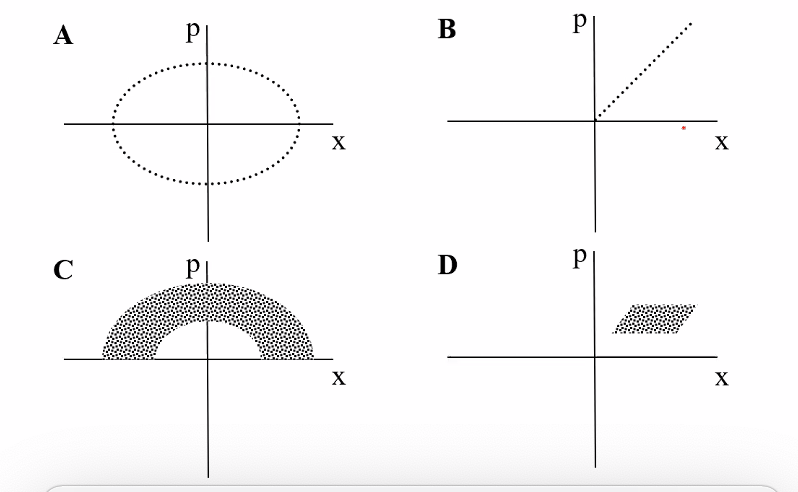
\includegraphics[scale=0.7]{Lecture-23/l23-img3.png}
\end{center}
\begin{s}
For a given fixed energy, we stay on the ellipse, and the phase angle just tells you where you are on the ellipse. So, A.
\end{s}
Consider an area element in phase space. What physically must happen for a particle to move into the area across the left boundary?
\begin{center}
    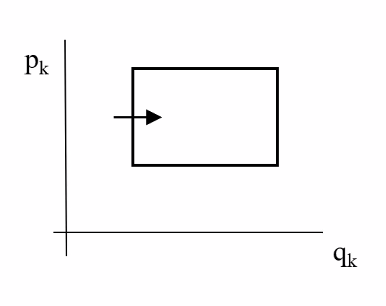
\includegraphics[scale=1]{Lecture-23/l23-img4.png}
\end{center}
\begin{s}
The position $q_k$ increases but the momentum $p_k$ is constant.
\end{s}

\subsubsection{Particle in a Central Force Field}
The kinetic energy for a particle of mass $m$ in a central force field is given by:
\[T = \frac{m}{2}\left(\dot{r}^2 + r^2\dot{\phi}^2\right)\]
Then we have the generalized momenta:
\[p_r = \dpd{T}{\dot{r}} = m\dot{r} \implies \dot{r} = \frac{p_r}{m}\]
\[p_\phi = \dpd{T}{\dot{\phi}} = mr^2\dot{\phi} \implies \dot{\phi} = \frac{p_\phi}{mr^2}\]
Hence the Hamiltonian has the form:
\[\HH = T + U = \frac{1}{2m}\left(p_r^2 + \frac{p_\phi^2}{r^2}\right) + U(r)\]
Hence Hamilton's equations yield:
\[\dot{r} = \dpd{\HH}{p_r} = \frac{p_r}{m}, \quad \dot{p}_r = -\dpd{\HH}{r} = \frac{p_\phi^2}{mr^3} - \dod{U}{r}\]\
\[\dot{\phi} = \dpd{\HH}{p_\phi} = \frac{p_\phi}{mr^2}, \quad p_\phi = -\dpd{\HH}{\phi} = 0\]
\subsubsection{General Procedure for setting up Hamilton's equations}
\begin{enumerate}[1.]
\item Choose suitable generalized coordinates, $q_{1}, \cdots, q_{n}$.
\item Write down the kinetic and potential energies, $T$ and $U$, in terms of the $q$ 's and $\dot{q}$ 's. 
\item Find the generalized momenta $p_{1}, \cdots, p_{n} .$ (We are now assuming our system is conservative, so $U$ is independent of $\dot{q}_{i}$ and we can use $p_{i}=\partial T / \partial \dot{q}_{i} .$ In general, one must use $p_{i}=\partial \mathcal{L} / \partial \dot{q}_{i}$. 
\item Solve for the $\dot{q}$ 's in terms of the $p$ 's and $q$ 's.
\item Write down the Hamiltonian $\mathcal{H}$ as a function of the $p$ 's and $q$ 's. [Provided our coordinates are "natural" (relation between generalized coordinates and underlying Cartesians is independent of time), $\mathcal{H}$ is just the total energy $\mathcal{H}=T+U,$ but when in doubt, use $\mathcal{H}=\sum p_{i} \dot{q}_{i}-\mathcal{L} .$ See Problems 13.11
and $13.12 .]$.
\item Write down Hamilton's equations (13.25).
\end{enumerate}
We will illustrate the advantages of using Hamilton's equations rather than Lagrange next week. One advantage is that we get first order versus second order equations, which can be easier sometimes (we have more techniques). A deeper advantage is theoretical, which we will see. We will also see how to construct a quantum theory with this framework.